\documentclass[aspectratio=169,9pt]{beamer}
\usetheme[progressbar=frametitle,numbering=fraction]{metropolis}
\usepackage[utf8]{inputenc}
\usepackage[T1]{fontenc}
\usepackage{amsmath,amssymb}
\usepackage{graphicx}
\usepackage{booktabs}
\usepackage{tabularx}
\usepackage{siunitx}
\usepackage{xcolor}
\sisetup{detect-all}
\definecolor{cRed}{HTML}{D62839}
\definecolor{cBlue}{HTML}{2A6FBB}
\definecolor{cGreen}{HTML}{2A9D55}
\definecolor{cOrange}{HTML}{E07B39}
\definecolor{tA}{HTML}{1F77B4}\definecolor{tB}{HTML}{FF7F0E}\definecolor{tC}{HTML}{2CA02C}\definecolor{tD}{HTML}{D62728}\definecolor{tE}{HTML}{9467BD}
\newcommand{\um}{\,\si{\micro\metre}}
\newcommand{\sw}[1]{\textcolor{#1}{\rule{1.6ex}{1.6ex}}}

\title{Multi-parameter clustering of the Ciona time-lapse}
\subtitle{$E$, $\alpha$, indentation $\delta$ and adhesion: what is independent, what clusters, what is interesting, and what to do next}
\date{41 force-volume maps, 17:15--21:48 (4.5\,h), 108\,790 valid pixels $\cdot$ controls: full map data\_213626}
\author{}

\begin{document}
\maketitle

\begin{frame}{Summary}
\scriptsize
\begin{enumerate}
\item \textbf{Yes, it makes sense, but only after removing what is not independent.} Of the 11 per-pixel quantities, about \textbf{four} carry their own information.
\item \textbf{$\delta$ adds almost nothing.} $\log\delta$ is $\SI{94}{\percent}$ explained by $\log E$ and $\alpha$. With the peak force and slope added ($\SI{97.7}{\percent}$), the Hertz scaling $\delta\propto(F/E)^{2/3}$ is recovered. Only the residual $\delta^*$ is kept.
\item \textbf{Adhesion: six numbers $\to$ two axes.} \emph{Strength} (force, work) and \emph{range} (short-range vs.\ long-range / tethers). \textcolor{cRed}{\textbf{But the adhesion force follows the peak (loading) force}} ($\rho=0.95$, $F_\mathrm{adh}\approx0.2\,F_\max$). The peak force is set by $E$ under a fixed ramp. The ``stiff = adhesive'' correlation ($\rho=0.54$) is therefore mostly a loading effect. The load-normalised adhesion $F_\mathrm{adh}/F_\max$ is almost independent of $E$ ($\rho=-0.12$).
\item \textbf{The data form a continuum, not discrete types.} The BIC keeps falling with $k$. $k=5$ is the most reproducible split beyond $k\le3$ (resampling ARI 0.88). The clusters are: soft/weak contact, soft/fluid-like, \textbf{tether-forming}, stiff/adhesive, stiff/solid-like.
\item \textbf{Interesting, and robust to the controls:}
\begin{itemize}\footnotesize
\item Clusters form \textbf{coherent domains} (same-label neighbours $\SI{66}{\percent}$ vs.\ $\SI{26}{\percent}$ by chance).
\item \textbf{Junctions are stiffer than cell centres.} $E$ was not used for segmentation.
\item \textbf{Tracked cells keep a mechanical identity over time}, even after removing tissue-scale trends (ICC 0.35--0.47).
\item Tethers form a distinct population ($\SI{9}{\percent}$ of pixels), concentrated on steep flanks.
\end{itemize}
\item \textbf{Main confounds:} the local slope of the surface, the peak force, the cell size ($\approx4$ px across), and the choice of model variant (cluster ARI 0.5--0.75 between variants).
\item \textbf{Has it been done?} Power-law $E$/$\alpha$ maps exist. Okajima \& Hotta labs have mapped ascidian embryos (single-cell stiffness and power-law rheology in cleavage stages). Clustering of multiparametric AFM maps exists for PeakForce-QNM data and cancer cells. \textbf{I found no study combining viscoelastic, adhesion and tether parameters with 3D registration and cell tracking in a live embryo time-lapse.}
\end{enumerate}
\end{frame}

% =====================================================================
\section{Data and features}

\begin{frame}{Per-pixel quantities}
\footnotesize
\begin{columns}[T]
\begin{column}{0.52\textwidth}
\begin{tabularx}{\linewidth}{@{}lX@{}}\toprule
quantity & source \\\midrule
$\log_{10}E_{1\,\mathrm{ms}}$ & Ting fit: $E(t)=E_1(t/t_0)^{-\alpha}$, evaluated at \SI{1}{ms} \\
$\alpha$ & power-law exponent (fluidity) \\
$\log_{10}\delta$ & maximum indentation \\
$F_\mathrm{adh}$, $\log W_\mathrm{adh}$ & adhesion force, work of adhesion \\
$L_\mathrm{adh}$, pull-off $z$ & detachment length, pull-off position \\
ruptures, tether & rupture events, tether present (plateau) \\
slope, height & local geometry (from topography) \\
\bottomrule\end{tabularx}
\end{column}
\begin{column}{0.45\textwidth}
\textbf{Preprocessing}
\begin{itemize}
\item The time-lapse maps store $E_1$ (at $t_0=\SI{1}{s}$), so $E_{1\,\mathrm{ms}}=E_1\cdot1000^{\alpha}$. This was checked against the pipeline's own $E_{1\,\mathrm{ms}}$ on data\_213626: equal to $10^{-7}$.
\item Only fits that pass the quality mask; 108\,790 of 125\,150 pixels.
\item \textbf{Per-frame robust standardisation} (median, MAD): removes the global drift over time ($E$ roughly doubles) so that clusters describe \emph{spatial} differences.
\item \textbf{Slope residualisation}: per frame, each feature minus a quadratic fit in the local slope.
\end{itemize}
\end{column}
\end{columns}
\end{frame}

\begin{frame}{Which quantities move together?}
\begin{columns}[T]
\begin{column}{0.5\textwidth}
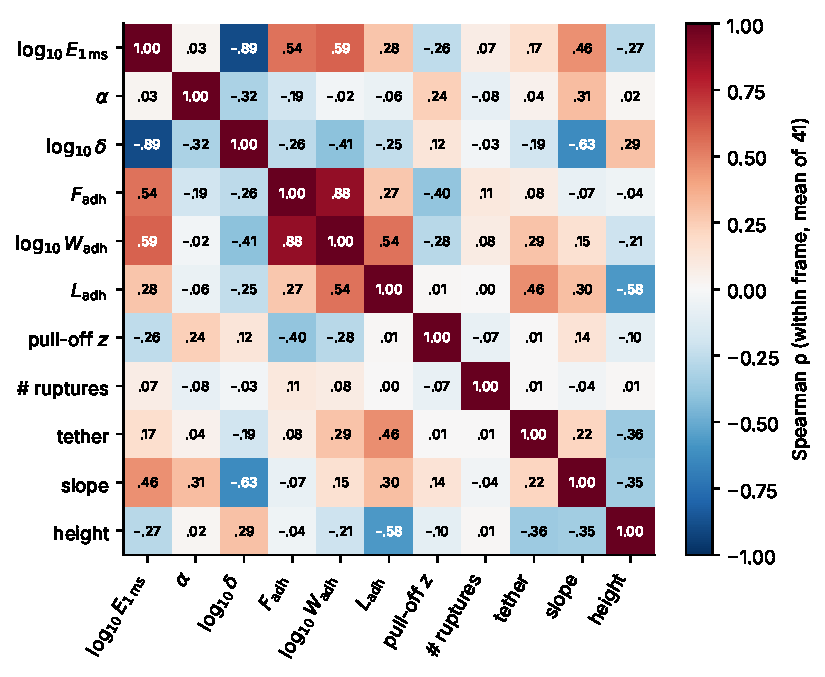
\includegraphics[width=\linewidth]{fig/corr_matrix.pdf}
\end{column}
\begin{column}{0.48\textwidth}\footnotesize
Spearman $\rho$ within each frame, averaged over the 41 frames:
\begin{itemize}
\item $\log E$ -- $\log\delta$: $-0.89$ $\Rightarrow$ $\delta$ is mostly $E$ (next slide).
\item $F_\mathrm{adh}$ -- $\log W$: $0.88$ $\Rightarrow$ one ``strength'' axis.
\item $\log E$ -- adhesion: $0.54$ / $0.59$ $\Rightarrow$ mostly via the peak force (see ``Caution'' slide).
\item $L_\mathrm{adh}$ -- tether: $0.46$. Long detachment = tethers.
\item \textbf{$\log E$ -- $\alpha$: $0.03$.} No overall correlation, but structure inside the clusters (see ``The five clusters'').
\item \textbf{Slope} correlates with $\log E$ ($0.46$), $\log\delta$ ($-0.63$), $\alpha$ ($0.31$), $L_\mathrm{adh}$ ($0.30$). Geometry is the largest confound.
\end{itemize}
\end{column}
\end{columns}
\end{frame}

\begin{frame}{Is the indentation $\delta$ an independent property? No.}
\begin{columns}[T]
\begin{column}{0.6\textwidth}
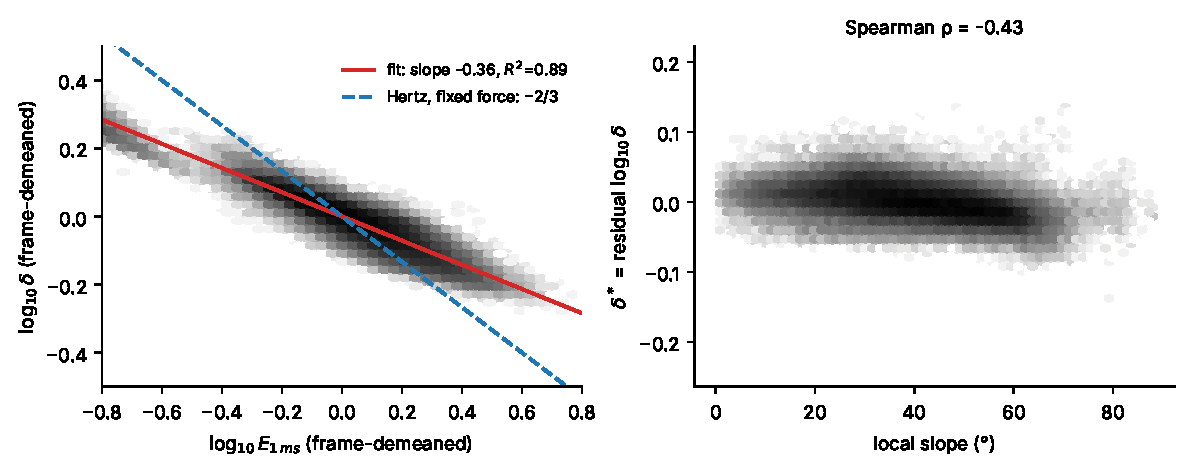
\includegraphics[width=\linewidth]{fig/delta_vs_E.pdf}
\end{column}
\begin{column}{0.38\textwidth}\footnotesize
Hertz (sphere): $F=\frac{4}{3}\frac{E}{1-\nu^2}\sqrt{R}\,\delta^{3/2}$ $\Rightarrow$ $\log\delta=\frac23(\log F-\log E)+c$.
\begin{tabular}{@{}lc@{}}\toprule
regressors of $\log\delta$ & $R^2$ \\\midrule
$\log E$ (time-lapse) & 0.89 \\
$\log E$, $\alpha$ (time-lapse) & 0.94 \\
$\log E$, $\log F_\max$, $\alpha$, slope (full map) & 0.977 \\
\bottomrule\end{tabular}\\[3pt]
On the full map, with $F_\max$ and slope included, the coefficients become $-0.69$ (on $\log E$) and $+0.57$ (on $\log F_\max$), close to $\mp\frac23$.\\[3pt]
\textbf{$\Rightarrow$ $\delta$ is a derived quantity.} Only its residual $\delta^*$ (what $E$, $\alpha$ do not explain) is used. $\delta^*$ still correlates with slope ($\rho=-0.43$), so it mainly carries contact geometry.
\end{column}
\end{columns}
\end{frame}

\begin{frame}{Adhesion: six numbers, two axes}
\footnotesize
\begin{columns}[T]
\begin{column}{0.52\textwidth}
PCA of the six adhesion quantities (frame-demeaned, standardised):\\[3pt]
\begin{tabular}{@{}lrrrrrr@{}}\toprule
& $F_\mathrm{adh}$ & $\log W$ & $L_\mathrm{adh}$ & pull-off & rupt. & tether \\\midrule
PC1 (\SI{40}{\percent}) & $-.53$ & $-.59$ & $-.39$ & $.33$ & $-.11$ & $-.33$\\
PC2 (\SI{27}{\percent}) & $.35$ & $.11$ & $-.56$ & $-.43$ & $.15$ & $-.58$\\
\bottomrule\end{tabular}\\[6pt]
\begin{itemize}
\item \textbf{adhesion strength} ($-$PC1): force, work, length, all larger.
\item \textbf{short- vs.\ long-range} (PC2): $+$ = strong short-range adhesion; $-$ = long detachment, tethers, late pull-off.
\item Rupture events are rare (mean 0.11 per curve). Tethers occur in \SI{9}{\percent} of the curves.
\end{itemize}
\end{column}
\begin{column}{0.45\textwidth}
\textbf{Interpretation}
\begin{itemize}
\item Strength $\approx$ contact area $\times$ adhesion energy (bonds, glycocalyx).
\item Range / tethers $\approx$ membrane mechanics: a tether forms when the membrane separates from the cortex. Its force is set by membrane tension and bending stiffness.
\item These two axes are what clustering uses for adhesion: \emph{adh.\ strength} and \emph{adh.\ short vs.\ long}.
\end{itemize}
\end{column}
\end{columns}
\end{frame}

\begin{frame}{Caution: the adhesion force follows the peak force}
\begin{columns}[T]
\begin{column}{0.64\textwidth}
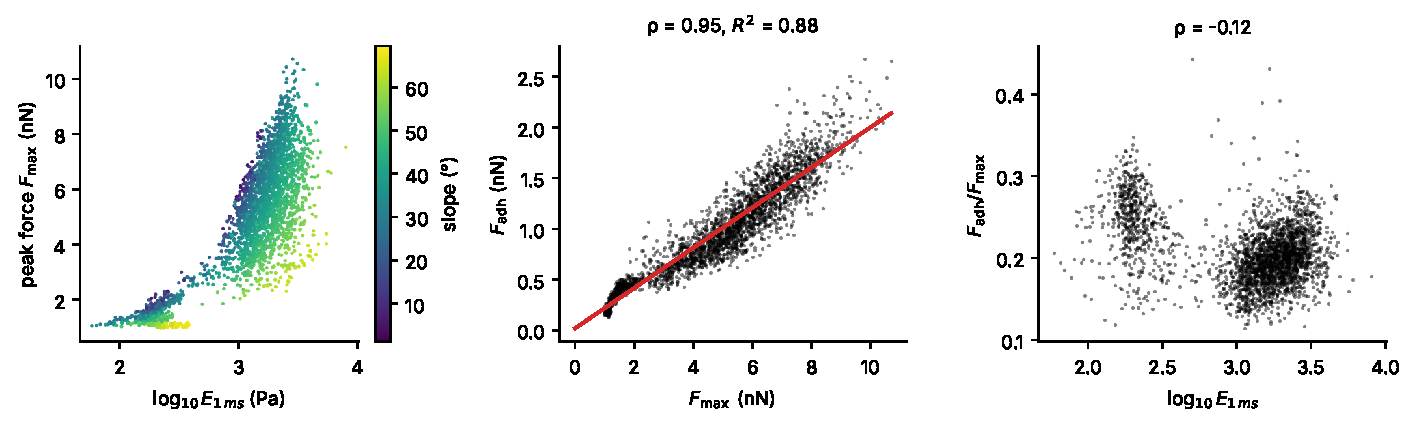
\includegraphics[width=\linewidth]{fig/fmax_confound.pdf}\\
\scriptsize Full map data\_213626 (2741 curves with $R^2>0.9$). Colour: local slope.
\end{column}
\begin{column}{0.34\textwidth}\footnotesize
\begin{itemize}
\item The peak force varies widely: 1.2 / 5.2 / 8.1\,nN (5/50/95\,\%). It follows $E$ ($\rho=0.74$), as expected for a fixed $z$ ramp.
\item $F_\mathrm{adh}\approx0.2\,F_\max$: $\rho=0.95$, $R^2=0.88$. Work: $\rho=0.80$.
\item Partial correlation $F_\mathrm{adh}$--$E$ given $F_\max$: only 0.32.
\item \textbf{The load-normalised adhesion} $F_\mathrm{adh}/F_\max$ (0.15--0.28) is almost independent of $E$ ($\rho=-0.12$) and $\alpha$ ($\rho=-0.06$).
\item Length, pull-off and tethers depend much less on the load ($|\rho|\le0.31$, except pull-off $-0.69$).
\end{itemize}
\textcolor{cRed}{The time-lapse maps contain no $F_\max$.} The extractor now exports \texttt{Fmax\_nN} and \texttt{adh\_ratio}, so the time-lapse can be redone after a re-export.
\end{column}
\end{columns}
\end{frame}

% =====================================================================
\section{Clustering}

\begin{frame}{Method and the number of clusters}
\begin{columns}[T]
\begin{column}{0.42\textwidth}
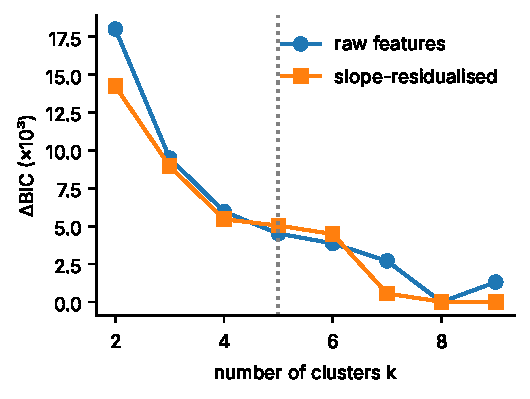
\includegraphics[width=\linewidth]{fig/bic.pdf}\\[4pt]
\footnotesize
\begin{tabular}{@{}lccccccc@{}}\toprule
$k$ & 2 & 3 & 4 & \textbf{5} & 6 & 7 & 8\\\midrule
ARI & .98 & .91 & .64 & \textbf{.88} & .72 & .77 & .61\\
\bottomrule\end{tabular}\\
\scriptsize Agreement between refits on independent subsamples (mean pairwise adjusted Rand index).
\end{column}
\begin{column}{0.56\textwidth}\footnotesize
\textbf{Features} (5): $\log E$, $\alpha$, $\delta^*$, adhesion strength, adhesion short vs.\ long. All per-frame robust $z$, slope-residualised.\\[3pt]
\textbf{Model}: Gaussian mixture, full covariance, fitted on 30\,000 random pixels, applied to all. Clusters are ordered by $\log E$.\\[3pt]
\textbf{Number of clusters}:
\begin{itemize}
\item The BIC keeps decreasing up to $k=9$: there is no natural number. The pixels form a \textbf{continuum}.
\item $k$ was therefore chosen by \textbf{reproducibility}. $k=2,3$ are trivially stable. $k=5$ is the stable split with more detail (ARI 0.88, minimum 0.83).
\item Refitting $k=5$ on five other subsamples: ARI 0.89--0.94 against the reported labels.
\end{itemize}
\textbf{Slope matters}: clusters on raw vs.\ slope-residualised features agree only with ARI 0.43.
\end{column}
\end{columns}
\end{frame}

\begin{frame}{The five clusters}
\begin{columns}[T]
\begin{column}{0.44\textwidth}
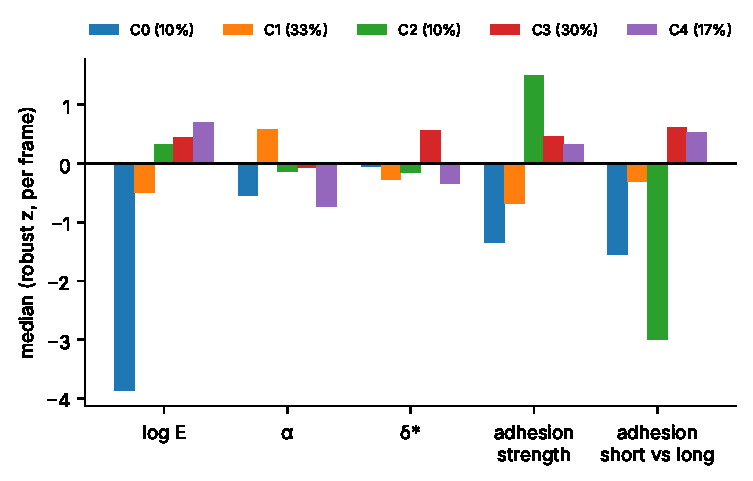
\includegraphics[width=\linewidth]{fig/profiles.pdf}
\end{column}
\begin{column}{0.55\textwidth}\scriptsize
\setlength{\tabcolsep}{3pt}
\begin{tabular}{@{}l@{\,}lrrrrrrr@{}}\toprule
& & \% & $E_{1\,\mathrm{ms}}$ & $\alpha$ & $\delta$ & $F_\mathrm{adh}$ & $L_\mathrm{adh}$ & teth.\\
& & & Pa & & \textmu m & nN & \textmu m & \%\\\midrule
\sw{tA}&C0 soft, weak & 10 & 217 & .49 & 3.0 & .45 & 3.5 & 5\\
\sw{tB}&C1 soft, fluid & 33 & 889 & .53 & 1.8 & .72 & 2.9 & 0\\
\sw{tC}&C2 tethers & 10 & 1500 & .52 & 1.5 & 1.01 & 7.3 & 85\\
\sw{tD}&C3 stiff, adhesive & 30 & 1381 & .50 & 1.7 & 1.16 & 3.3 & 0\\
\sw{tE}&C4 stiff, solid & 17 & 1541 & .50 & 1.5 & 1.00 & 3.6 & 0\\
\bottomrule\end{tabular}\\[2pt]
Medians in physical units. The median slope is 36--42° except for C2 (51°) and C4 (47°).\\[4pt]
\footnotesize
\begin{itemize}
\item The \textbf{$E$--$\alpha$ trade-off} appears between C1 (softer, higher $\alpha$) and C4 (stiffer, lower $\alpha$). This matches ``stiffer = less fluid'' in single cells. Overall $\rho\approx0$ because C0 is soft \emph{and} has low $\alpha$.
\item \textbf{C2} is defined by tethers and long detachment. It is the most distinct cluster.
\item \textbf{C0}: very soft, deep indentation, weak adhesion; large patches at the edge of the last frames. Possibly a different surface (another cell type, test cells) or partial contact.
\item Absolute $\alpha$ differences are small (0.49--0.53). $\alpha$ is reliable only in relative terms (see the variants deck).
\end{itemize}
\end{column}
\end{columns}
\end{frame}

\begin{frame}{Cluster structure in feature space}
\centering
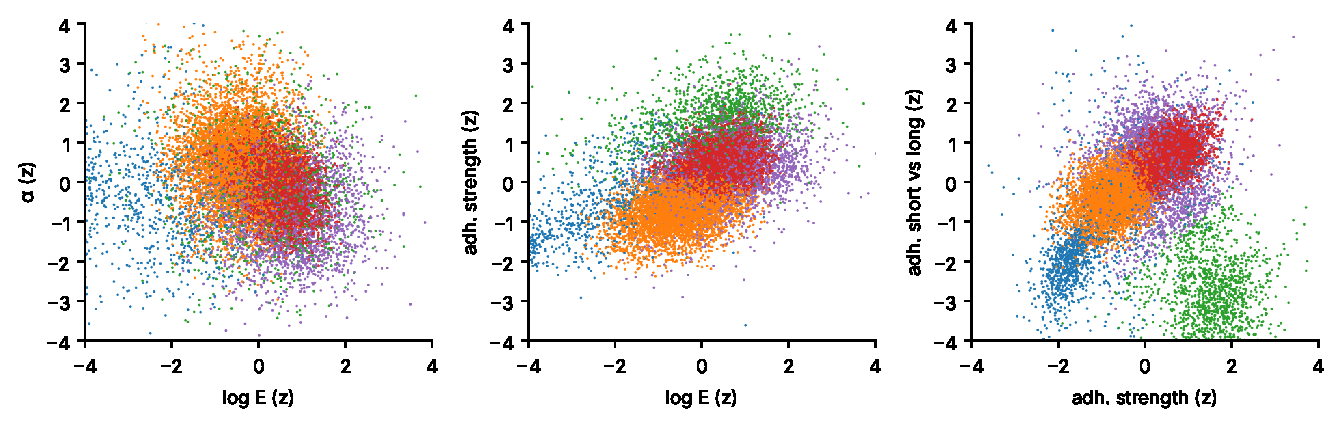
\includegraphics[width=0.95\linewidth]{fig/scatter_clusters.pdf}\\
\footnotesize 15\,000 random pixels, colours as on the previous slide. The clusters are regions of one continuous cloud, except for the tether population (green, low ``short vs.\ long'').
\end{frame}

% =====================================================================
\section{Where are the clusters?}

\begin{frame}{Cluster maps (scan coordinates)}
\centering
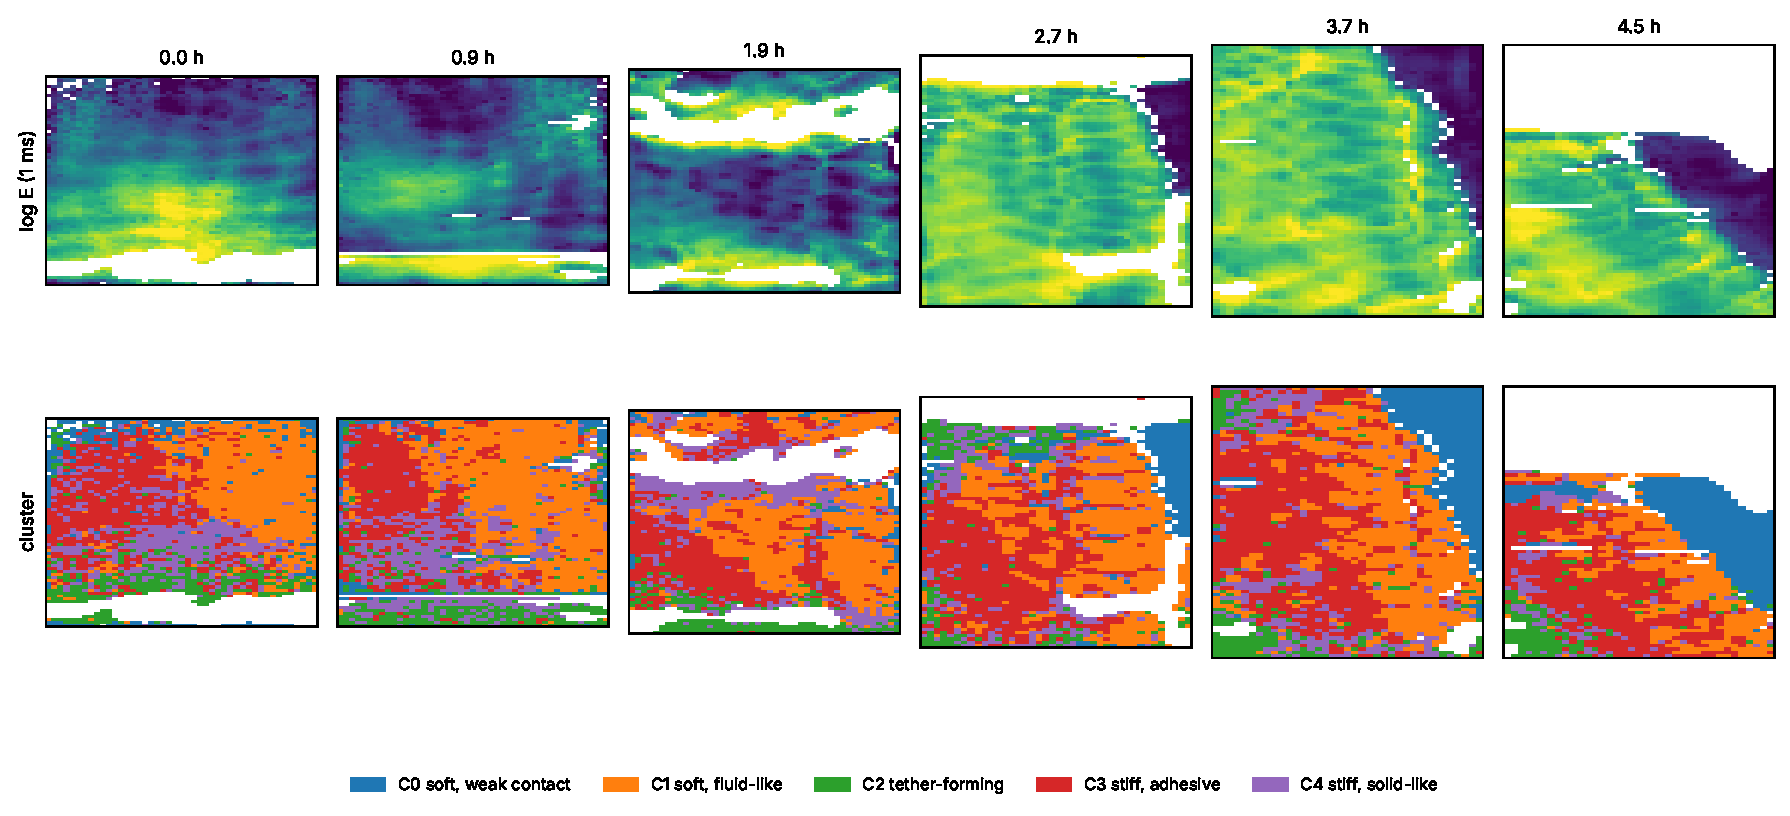
\includegraphics[width=\linewidth]{fig/cluster_maps.pdf}\\
\footnotesize Top: $\log E_{1\,\mathrm{ms}}$. Bottom: cluster. White: no valid fit. Same-label neighbour fraction \textbf{0.66} vs.\ 0.26 for spatially random labels: the clusters form \textbf{coherent domains}, several cells wide.
\end{frame}

\begin{frame}{Cluster maps on the registered 3D surface}
\centering
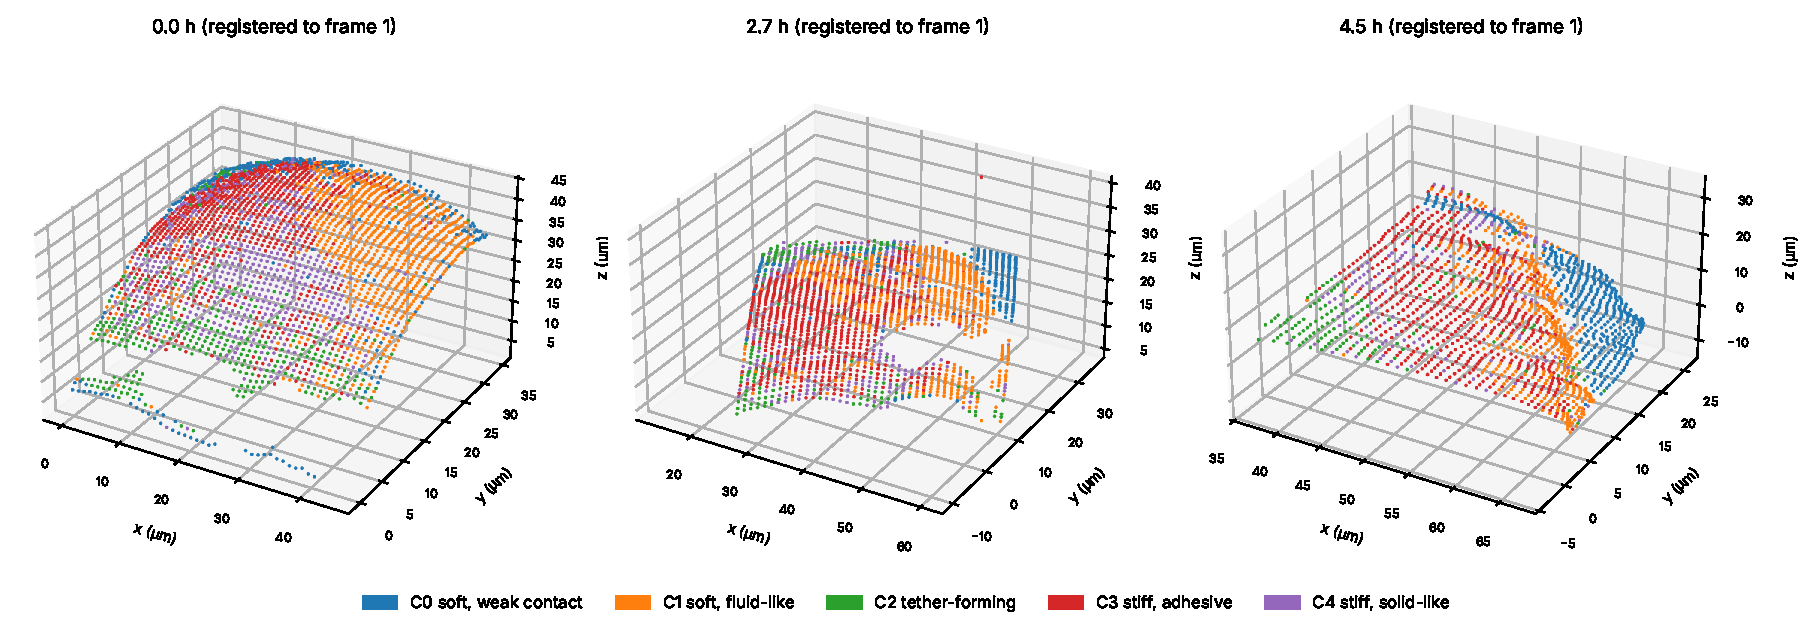
\includegraphics[width=\linewidth]{fig/cluster_3d.pdf}\\
\footnotesize Each frame transformed into the coordinates of frame 1 (rigid 3D registration, chained). Tethers (green) gather on the steep lower flank. The stiff clusters (red, purple) sit on the crest.
\end{frame}

\begin{frame}{Where in the embryo frame do clusters occur, over all 41 frames?}
\centering
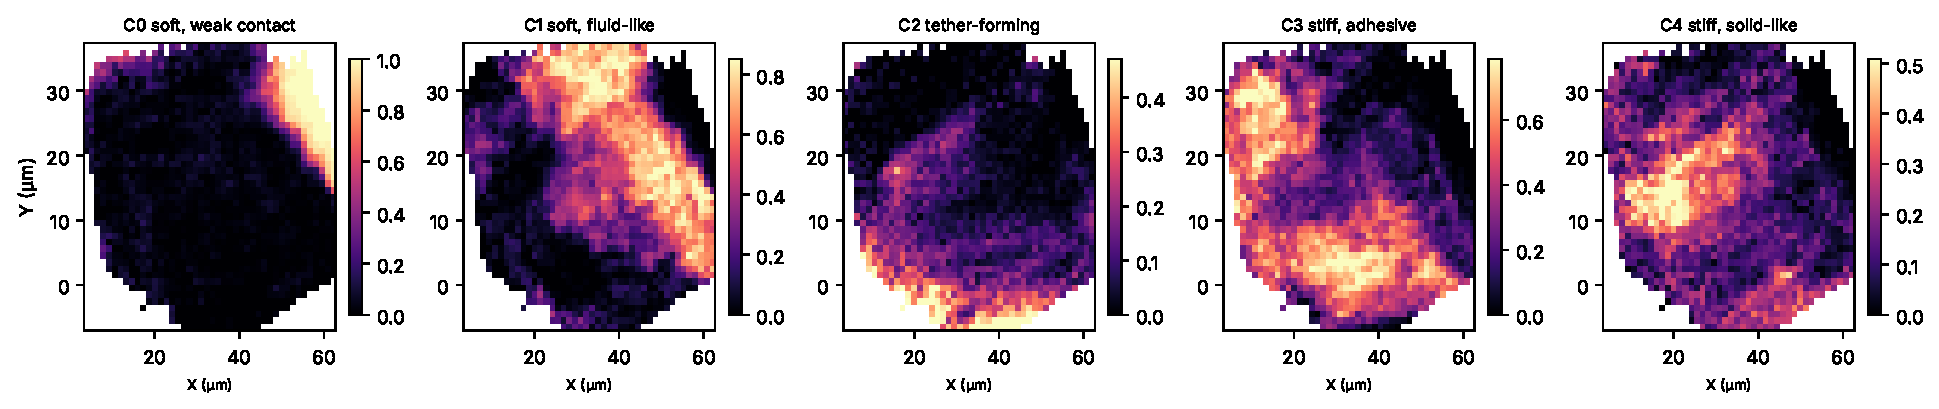
\includegraphics[width=\linewidth]{fig/occupancy_registered.pdf}\\[2pt]
\footnotesize Fraction of pixels in each cluster per $\approx\SI{1.3}{\micro\metre}$ bin, all frames pooled in registered coordinates.
C0 occupies one edge (the soft region that dominates the last frames). C1 and C3 split the central surface. C2 lies along the lower flank.
Correlation lengths of the features ($1/e$ of the spatial autocorrelation): $\log E$ and $\alpha$ \SI{5}{\micro\metre}, adhesion strength \SI{6.5}{\micro\metre}, $\delta^*$ and adhesion range 2.5--\SI{3}{\micro\metre}. These are cell-sized or larger ($\approx\SI{4.4}{\micro\metre}$ cells).
\end{frame}

\begin{frame}{How the composition changes over 4.5\,h}
\begin{columns}[T]
\begin{column}{0.55\textwidth}
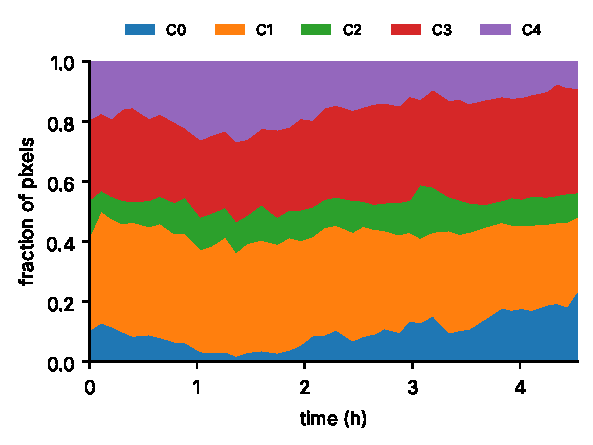
\includegraphics[width=\linewidth]{fig/fractions_time.pdf}
\end{column}
\begin{column}{0.43\textwidth}\footnotesize
\begin{itemize}
\item Features are standardised per frame, so this shows \emph{relative} composition, not the global stiffening.
\item First 0.4\,h $\to$ last 0.4\,h: C1 (soft, fluid) $36\to27\,\%$, C3 (stiff, adhesive) $28\to35\,\%$, C4 (stiff, solid) $17\to9\,\%$ (peak $24\,\%$ at 0.9--1.7\,h).
\item C0 (soft, weak contact): $11\,\%$ at the start, $3\,\%$ at 0.9--1.7\,h, then $19\,\%$ at the end, when the soft region enters at the edge.
\item Tethers (C2) stay at 8--11\,\%.
\item \textbf{The field of view moves over the embryo}, so composition changes mix development with sampling a different part of the surface. Per-cell tracking (next section) separates the two.
\end{itemize}
\end{column}
\end{columns}
\end{frame}

% =====================================================================
\section{Cell scale}

\begin{frame}{From junction to cell centre}
\begin{columns}[T]
\begin{column}{0.62\textwidth}
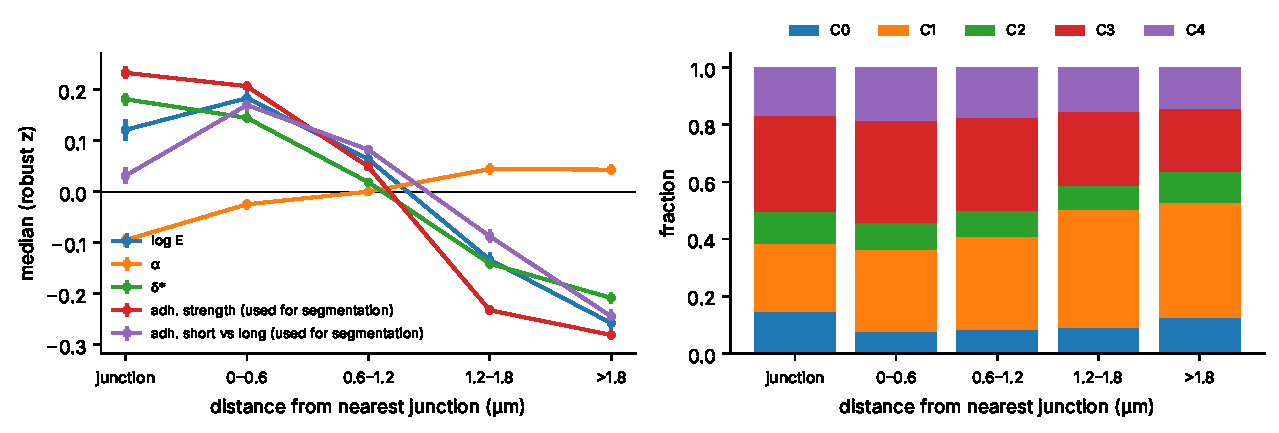
\includegraphics[width=\linewidth]{fig/junction_profiles.pdf}
\end{column}
\begin{column}{0.36\textwidth}\footnotesize
Pixels binned by distance to the nearest segmented junction:
\begin{itemize}
\item \textbf{$\log E$: junction $+0.12$ to $+0.18$, centre $-0.26$} (robust $z$). Junctions and their surroundings are stiffer. $E$ was \emph{not} used for segmentation.
\item $\alpha$ is slightly lower at junctions ($-0.10$ vs.\ $+0.04$): less fluid.
\item Composition: C3 (stiff, adhesive) 34--36\,\% near junctions vs.\ 22\,\% at centres; C1 (soft, fluid) 24\,\% vs.\ 40\,\%.
\item \textcolor{cRed}{Caveats}: adhesion \emph{was} used to find junctions, so its profile is partly circular. Junctions are grooves, where contact geometry also changes the apparent $E$.
\end{itemize}
\end{column}
\end{columns}
\end{frame}

\begin{frame}{Do cells keep a mechanical identity over time?}
\begin{columns}[T]
\begin{column}{0.48\textwidth}
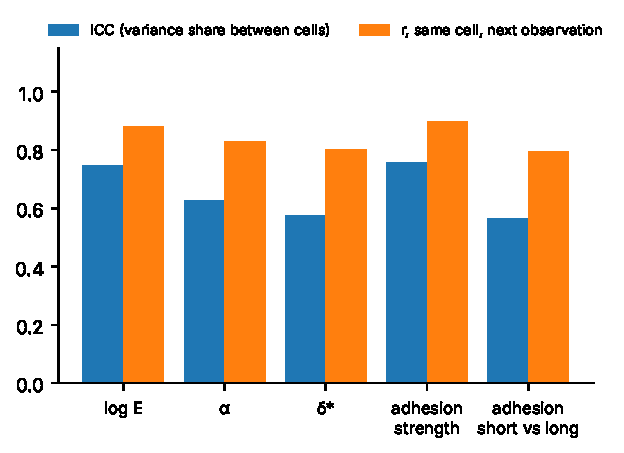
\includegraphics[width=\linewidth]{fig/cell_identity.pdf}\\
\scriptsize 367 tracks observed in $\ge4$ frames, 4126 cell observations. Frame effects removed.
\end{column}
\begin{column}{0.5\textwidth}\footnotesize
\textbf{ICC}: share of the variance of cell medians that lies \emph{between} cells rather than within a cell over time.\\[3pt]
\setlength{\tabcolsep}{3pt}
\begin{tabular}{@{}lccccc@{}}\toprule
& $\log E$ & $\alpha$ & $\delta^*$ & adh.\,str. & adh.\,range\\\midrule
ICC & .75 & .63 & .57 & .76 & .57\\
$r$ (next frame) & .88 & .83 & .80 & .90 & .80\\
ICC, detr.\ \SI{6}{\micro\metre} & .47 & .45 & .35 & .38 & .39\\
ICC, detr.\ \SI{3}{\micro\metre} & .34 & .28 & .24 & .27 & .26\\
\bottomrule\end{tabular}\\[4pt]
\begin{itemize}
\item The raw ICC partly reflects \emph{where} a cell is (tissue-scale domains).
\item Subtracting a Gaussian-smoothed field ($\sigma=6$ or \SI{3}{\micro\metre}) before taking cell medians removes the neighbourhood. A clear \textbf{cell-specific component remains}. Cells differ from their neighbours consistently over $\ge$\,20\,min.
\end{itemize}
\end{column}
\end{columns}
\end{frame}

\begin{frame}{Mechanics around cell division (tentative)}
\begin{columns}[T]
\begin{column}{0.52\textwidth}
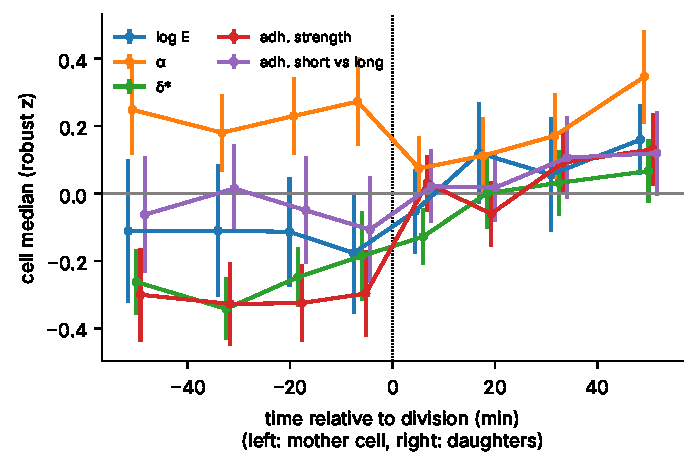
\includegraphics[width=\linewidth]{fig/division.pdf}
\end{column}
\begin{column}{0.46\textwidth}\footnotesize
63 confirmed divisions (mother track ends, two daughter tracks start). Cell medians aligned on the first daughter frame.\\[3pt]
Paired test, mother (last 3 frames) vs.\ daughters (first 3 frames), $n=59$, Wilcoxon:
\begin{itemize}
\item adhesion strength $-0.34\to-0.11$, $p=0.010$; range $p=0.011$; $\delta^*$ $p=0.037$.
\item $\log E$: $p=0.21$; $\alpha$: $p=0.09$. No significant change.
\end{itemize}
Only adhesion strength and range stay below 0.05 after a Bonferroni correction for 5 features ($p<0.01$ required: borderline).\\[3pt]
\textbf{Not conclusive.} Cells are $\approx4$ pixels across. A ``division'' is a segmentation split, not confirmed by imaging. Single-cell work in cleavage-stage ascidian embryos found stiffening and lower fluidity towards division. Resolving that here needs finer pixels and faster frames.
\end{column}
\end{columns}
\end{frame}

\begin{frame}{How much does the clustering depend on the Ting model variant?}
\footnotesize
Full map data\_213626, Gaussian mixture on the same features, computed from each model variant of $E_{1\,\mathrm{ms}}$ and $\alpha$. Agreement with the main fit (ARI, 1 = identical):\\[4pt]
\centering
\begin{tabular}{@{}lccc@{}}\toprule
features & vertical (no slope corr.) & squeeze film & lab contact point\\\midrule
$\log E$, $\alpha$, adhesion ($k=4$) & 0.75 & 0.58 & 0.51\\
$\log E$, $\alpha$ only ($k=3$) & 0.62 & 0.61 & 0.46\\
\bottomrule\end{tabular}\\[6pt]
\raggedright
\begin{itemize}
\item The clusters are \textbf{moderately model-dependent}, mainly through $\alpha$. $\alpha$ is the quantity most sensitive to the contact point and the toe force (see the variants deck).
\item Conclusions that rely on $E$ contrast and adhesion range are robust. Conclusions that rely on fine $\alpha$ differences need the toe resolved (speed series or dwell measurement).
\end{itemize}
\end{frame}

% =====================================================================
\section{Prior work}

\begin{frame}{Has anyone done this before?}
\scriptsize
\begin{tabularx}{\linewidth}{@{}>{\raggedright\arraybackslash}p{0.28\linewidth}X@{}}\toprule
work & relation to this analysis\\\midrule
Hecht et al., \emph{Soft Matter} 11, 4584 (2015) & First AFM maps of power-law exponent and modulus on live cells (force clamp). Stiffer cells consistently show a smaller exponent. Same $E$--$\alpha$ trade-off as C1 vs.\ C4.\\
Sanchez, Espinosa, Miguez, Garcia, \emph{Nanoscale} 13, 16339 (2021) & Power-law (fluidity) maps from force--distance curves, with finite-thickness correction. Local variations within single cells.\\
Fujii et al., \emph{Commun.\ Biol.} (2021), doi:10.1038/s42003-021-01869-w & AFM topography + stiffness of single cells in ascidian embryos, fertilised egg to pre-gastrula. Cells identified with the 3D virtual embryo.\\
Kotani et al., \emph{Biophys.\ J.} 124, 3139 (2025) & Single-cell power-law rheology in cleavage-stage ascidian embryos: higher modulus and lower fluidity towards division; three rheological states.\\
bioRxiv 2026.01.23.701227 & Rheology of the vegetal hemisphere of ascidian embryos (``breakdown of rheological universality'').\\
JSAP 2024 abstract 20a-P03-5 & AFM on tailbud ascidian embryos: elasticity gradient along tail elongation, abolished by myosin inhibition.\\
Thompson et al., \emph{eLife} 8, e39356 (2019) & Time-lapse \emph{in vivo} AFM of the \emph{Xenopus} brain: stiffness gradients form within tens of minutes.\\
Weber, Vivanco, Toca-Herrera, \emph{Sci.\ Rep.} 13, 3087 (2023) & Unsupervised self-organising maps + $k$-means on viscoelastic parameters of cancer cells.\\
\emph{Sensors} 23, 4730 (2023) & Clustering and manifold learning of PeakForce-QNM multiparametric maps (adhesion, modulus, \ldots).\\
\emph{Soft Matter} (2026), doi:10.1039/d5sm00943j & $k$-means and supervised classification of AFM force curves of soft nanoparticles.\\
\bottomrule\end{tabularx}
\end{frame}

\begin{frame}{What seems new here}
\footnotesize
As far as I could find (not an exhaustive review):
\begin{itemize}
\item \textbf{Joint clustering of viscoelastic ($E$, $\alpha$), indentation and adhesion/tether parameters} on a living embryo. Prior embryo AFM reports stiffness and/or power-law rheology, but not adhesion and tethers as further axes.
\item \textbf{Registered 3D surface + cell tracking}: following the same cells' mechanics over 4.5\,h, with tissue-scale trends separated from cell identity (detrended ICC).
\item \textbf{Systematic check of which parameters are independent}: $\delta$ is derived; adhesion follows the peak force. Multiparametric AFM clustering studies usually treat all channels as independent.
\item \textbf{Model-variant sensitivity of the clusters}.
\end{itemize}
The ascidian AFM work of the Okajima and Hotta groups is the closest. It covers earlier stages (cleavage), larger cells, and stiffness/rheology only. It is the natural reference for the stage, the method and the cell identity (FABA / 3D virtual embryo).
\end{frame}

% =====================================================================
\section{Where to go from here}

\begin{frame}{Caveats to address first}
\footnotesize
\begin{enumerate}
\item \textbf{Peak force.} Re-export the time-lapse with \texttt{Fmax\_nN} and \texttt{adh\_ratio} (now in the extractor). Cluster on load-normalised adhesion. Better still, use force-triggered acquisition (constant peak force) for future maps.
\item \textbf{Geometry.} Slope still drives $\delta^*$, tethers and part of $E$. Options: a curvature-aware contact model (sphere on a curved surface), restricting to flat regions, or adding slope and curvature as covariates in a hierarchical model.
\item \textbf{Resolution.} Cells are $\approx4$ pixels across at $1.0\times\SI{0.5}{\micro\metre}$. Finer pixels (0.25--\SI{0.5}{\micro\metre}) on smaller fields would make junction/centre and division analyses much stronger.
\item \textbf{Pixel size per frame} is still assumed (see the how-to). Rerun the extractor to write \texttt{pixels.json}.
\item \textbf{Specimen and stage.} Confirm what is scanned (embryo epidermis vs.\ test cells; chorion?), the hours post fertilisation and the temperature.
\end{enumerate}
\end{frame}

\begin{frame}{Next steps: analysis}
\footnotesize
\begin{enumerate}
\item \textbf{Per-cell, not per-pixel, phenotypes.} Cluster the tracked cells (medians, junction/centre contrast, time slopes). Test whether the groups are spatially ordered (rows, bands), as lineage-restricted epidermal rows would predict.
\item \textbf{Spatially aware clustering}: a Gaussian mixture with a Markov random field (Potts) prior. It uses neighbour coherence and reduces noise-driven speckle.
\item \textbf{Curve-shape learning}: cluster the force curves themselves (functional PCA or an autoencoder on approach + retract). This avoids model choices and can find features the Ting model misses, such as the toe or rupture patterns.
\item \textbf{Dynamics}: per-cell trajectories in ($E$, $\alpha$, adhesion) space. Test for state switching (hidden Markov model) and for lead--lag relations between neighbours, i.e.\ mechanical waves.
\item \textbf{Tethers $\to$ membrane tension}: $T = f_t^2/(8\pi^2\kappa)$ from the tether force $f_t$ (bending rigidity $\kappa$ assumed). This gives a tension map, independent of $E$ and directly comparable with other methods.
\end{enumerate}
\end{frame}

\begin{frame}{Next steps: experiments}
\footnotesize
\begin{enumerate}
\item \textbf{Perturbations} to give the axes a biological meaning:
\begin{itemize}\footnotesize
\item blebbistatin / ROCK inhibitor (myosin) $\to$ $E$ and $\alpha$;
\item latrunculin / cytochalasin (actin) $\to$ $E$, tethers;
\item methyl-$\beta$-cyclodextrin or osmotic shocks $\to$ membrane tension and tethers.
\end{itemize}
\item \textbf{Speed series or dwell / stress relaxation} on the same pixels: resolves the toe and pins $\alpha$ (the weakest axis).
\item \textbf{Correlative imaging}: membrane and actin markers, or bright field with the 3D virtual embryo (FABA), to name the cells and tissues behind the clusters.
\item \textbf{Several embryos and stages} with the same protocol. Are the five clusters, the junction stiffening and cell identity reproducible? This turns the analysis from descriptive into comparative.
\end{enumerate}
\end{frame}

\begin{frame}[fragile]{Reproduce}
\footnotesize
Scripts in \texttt{docs/clustering/scripts/} (paths are those of the analysis machine):
\begin{tabularx}{\linewidth}{@{}lX@{}}\toprule
\texttt{c1\_load.py} & pixel table from the extracted maps + registration \\
\texttt{c2\_stats.py} & correlations, $\delta$ regression, adhesion PCA, slope dependence \\
\texttt{c3\_cluster.py}, \texttt{c3b\_stab.py} & Gaussian mixture, BIC, stability, profiles, composition over time \\
\texttt{c4\_maps.py} & 2D, registered-3D and occupancy maps \\
\texttt{c5\_cells.py} & junction profiles, cell identity (ICC), correlation lengths \\
\texttt{c6\_controls.py} & detrended ICC, model-variant ARI \\
\texttt{c7\_division.py} & division-aligned mechanics \\
\texttt{c8\_fmax.py} & peak-force dependence of adhesion (full map) \\
\bottomrule\end{tabularx}\\[4pt]
Numbers quoted in the slides: \texttt{facts\_*.json}.
\end{frame}

\end{document}
